% LaTeX Präsentationsvorlage (2013) der TU Graz, rev12, 2013/01/31
\documentclass{beamer}
% \documentclass[aspectratio=169]{beamer}
%\usetheme{tugraz2013}
 \usetheme[notes]{tugraz2013}
% \usetheme[minimal]{tugraz2013}

%% Titelblatt-Einstellungen
\title[Android Bluetooth Credential Store]{Android Bluetooth \\ Credential Store}
\author{Camilla Reis}
% \date{Graz, XX. Dezember 2010}		% \today für heutiges Datum verwenden
\date{Graz, 7. November 2018}
\institute[IAIK]{\\ Institute of Applied Information Processing and Communications}
\instituteurl{www.tugraz.at}
% \institutelogo{kurz.pdf}
% \additionallogo{institutslogo.pdf}

%% Präsentationszeit: 15-20min 

\usepackage{hyperref}
\def\UrlBreaks{\do\/\do-}

%%%%%%%%%%%%%%%%%%%%%%%%%%%%%%%%%%%%%%%%%%%%%%%%%%%%%%%%%%%%%%%%%%%%%%%%%%%%
\begin{document}
%%%%%%%%%%%%%%%%%%%%%%%%%%%%%%%%%%%%%%%%%%%%%%%%%%%%%%%%%%%%%%%%%%%%%%%%%%%%
\titleframe

\begin{frame}
	\centering
	\vfill
	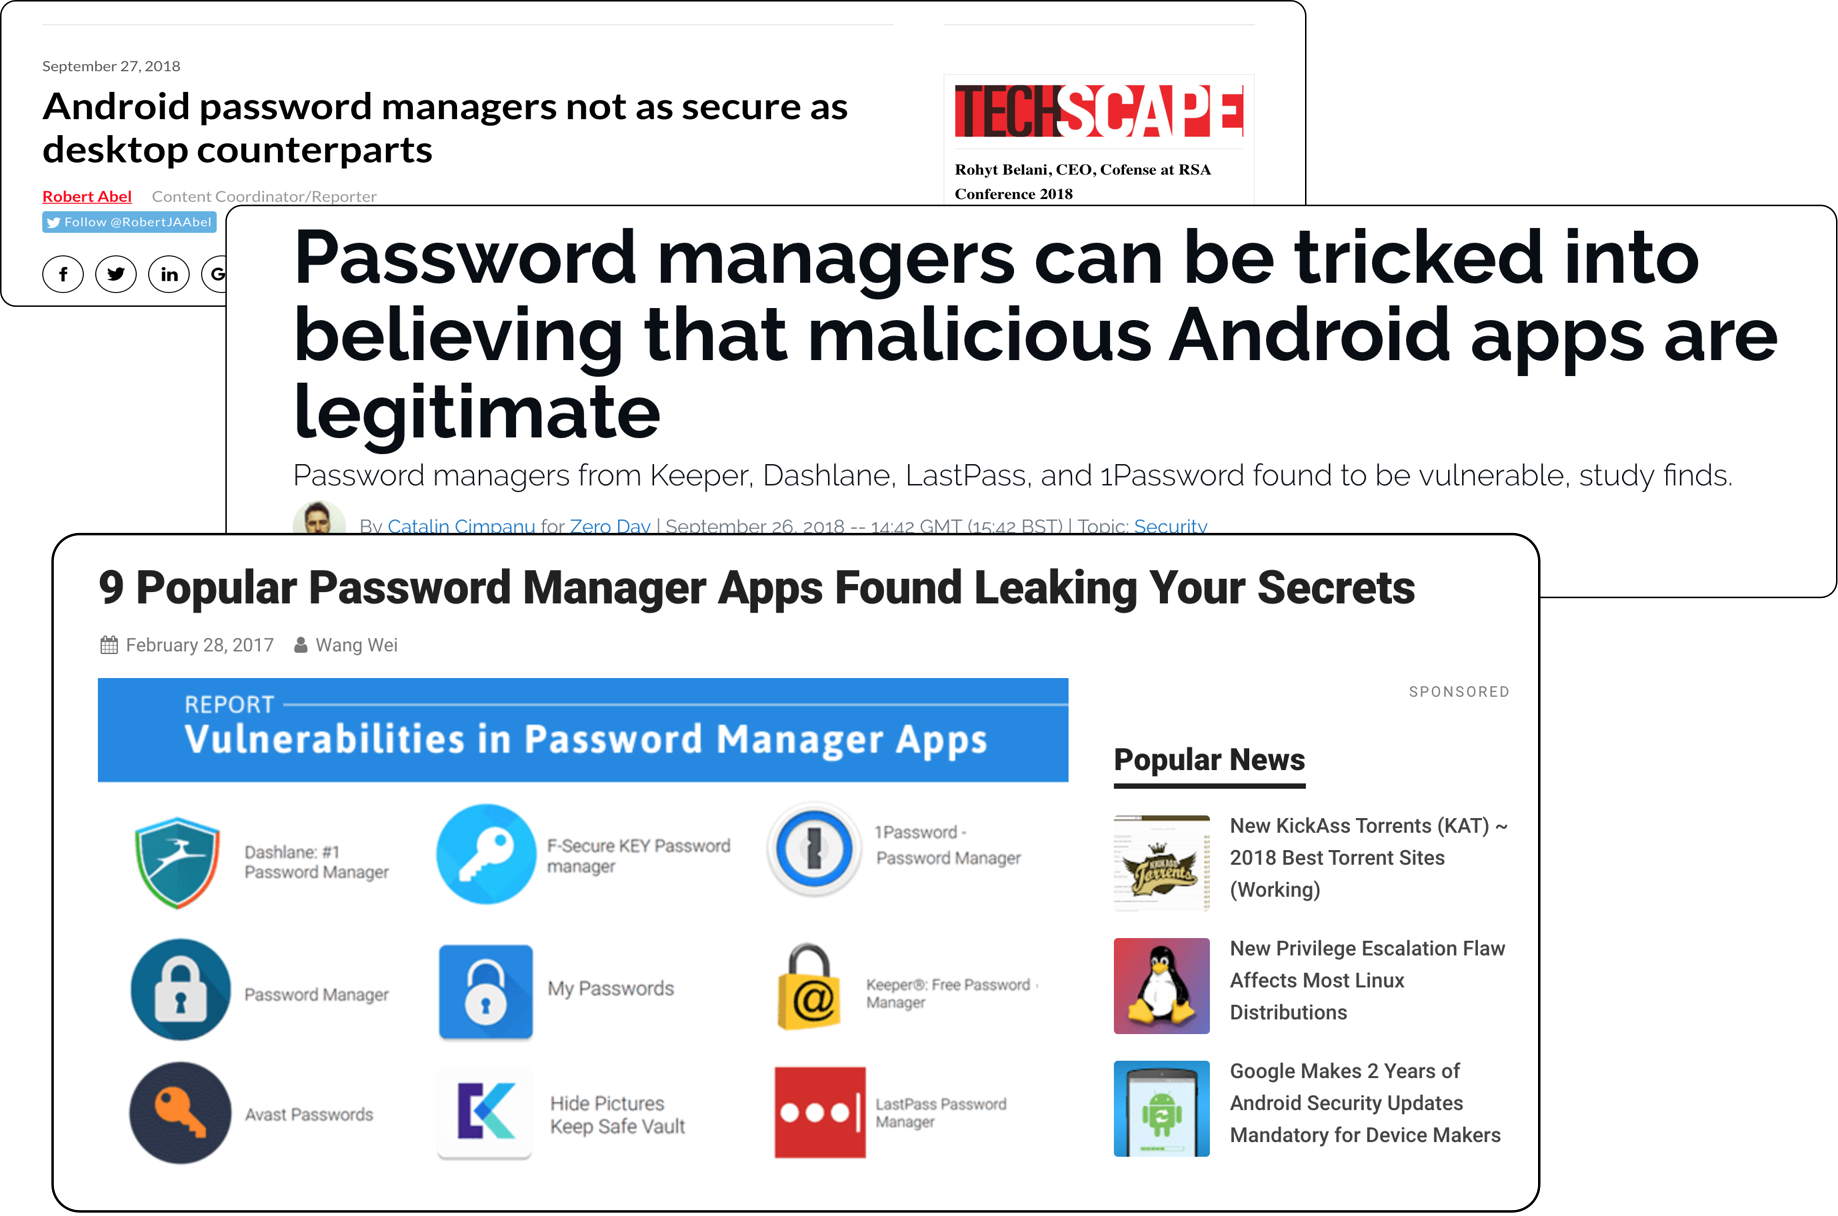
\includegraphics[width=1\textwidth]{images/papers.png}
	\vfill
%
\note{
aft. research many sources found that claim password managers are not as secure might seem. \\
Articles state: andr. pm less secure than desktop \& popular pm leaking secrets. \\
Have researched and found common problem with pm and developed a solution. \\}
\end{frame}



\section{Motivation}
\begin{frame}{Existing Solutions}
	\begin{itemize}
		\item Android applications prone to phishing attacks.
		\item Master passwords stored in plain text.
		\item Sniffing data from uncleaned clipboard.
		\item Web-based password managers use cookies for authentication.
	\end{itemize}
%
\note{
some recent vulnerabilities: popular pm prone exploitation through phishing.\\
Mali. applications phished cred by misleading the pm with tampered package. \\ User logs in, communicate backend. pm identifies with package. malic. app mimic legitimate app \\
MPassword in plain text. In case attack result in compromise of security \\
Sniffing of the phones clipboard. if not cleaned properly after copied, access credentials \\
Also web-based pm vulner. to attack cookies to authenticate user. \\
Although informed \& problems resolved, future vulnera. cannot be excluded. (3m)\\}
\end{frame}



\begin{frame}{Motivation of Project}
\vspace{-5mm}
\begin{itemize}
	\item The Android platform offers
	\begin{itemize}
		\item Trusted Execution Environment (TEE)
		\item Biometric authentication methods
		\item Android Permission System
		\item Sandboxing
	\end{itemize}
	\item Smartphones support our everyday life.
\end{itemize}
%
\note{
Now it might seem A. pwm just not secure. Nevertheless, we found Android system offers important sec. mechan. to provide integr, confi, authenti \\
Including: TEE, provide a secure hardware-backed solution to store sensitive data \\
Biometric Authentication Methods like Fingerprint. \\
Andr. Permi.System: most impor. sets restrictions and protects system resouces \\
Additionally, Sandboxing. offers advan. Linux user-based protection to identify \& isolate app resources. \\
Mobile phones support everyday, make data available. This makes ideal to store data. \\}
\end{frame}

\begin{frame}{Motivation of Project}
\vspace{-5mm}
\begin{itemize}
	\item Availability of credentials is important.
	\item Third parties compromise confidentiality.
	\item Our goal is to
	\begin{itemize}
		\item provide secure storage and availability of credentials.
		\item reduce external dependencies to increase confidentiality.
	\end{itemize}
\end{itemize}
%
\note{
Availability import. multiple devices. solution: synchronizing w/ cloud services. countless applications offer cloud services. store on servers owned by, access over Internet. cloud services compromise data confidentiality. Conf: accessed only authorized party. storing data on servers, unauthorized access, renounce cloud, avail. challenging.\\
Depending third-parties lead compromised security. Implementation weaknesses  and insecure handling lead vulnerabilities. goal to reduce external dependencies altogether. unexplored approach of sending credentials directly BT. data stored on phone: Authenticity provided. third parties excluded, risk compromised conf. reduced \\}
\end{frame}



\begin{frame}{Motivation of Project}
\begin{itemize}
	\item Solution:
	\begin{itemize}
		\item Android credential manager 
		\item Google Chrome extension
		\item Bluetooth LE connection for data transfer
		\item Data is stored on device
		\item Authentication is done via fingerprint
	\end{itemize}
\end{itemize}
%
\note{
Achieve goal, designed android credential manager, an accompanying Google ext, uses the web bt API: websites communicate BLE devices. \\
both establish BLE connection to transfer. data on device, selec cred shared on demand. to access/send user authenticate via, this ensures regis. fingerp., extension fills uname and pw into proper forms \\
7:30}
\end{frame}


%%%%%%%%%%%%%%%%%%%%%%%%%%%%%%%%%%%%%%%%%%%%%%%%%%%%%%%%%%%%%%%%%%%%%%%%%%%%

\section{Architecture of Project}

\begin{frame}{Workflow of Devices}
\vspace{-3mm}
\centering
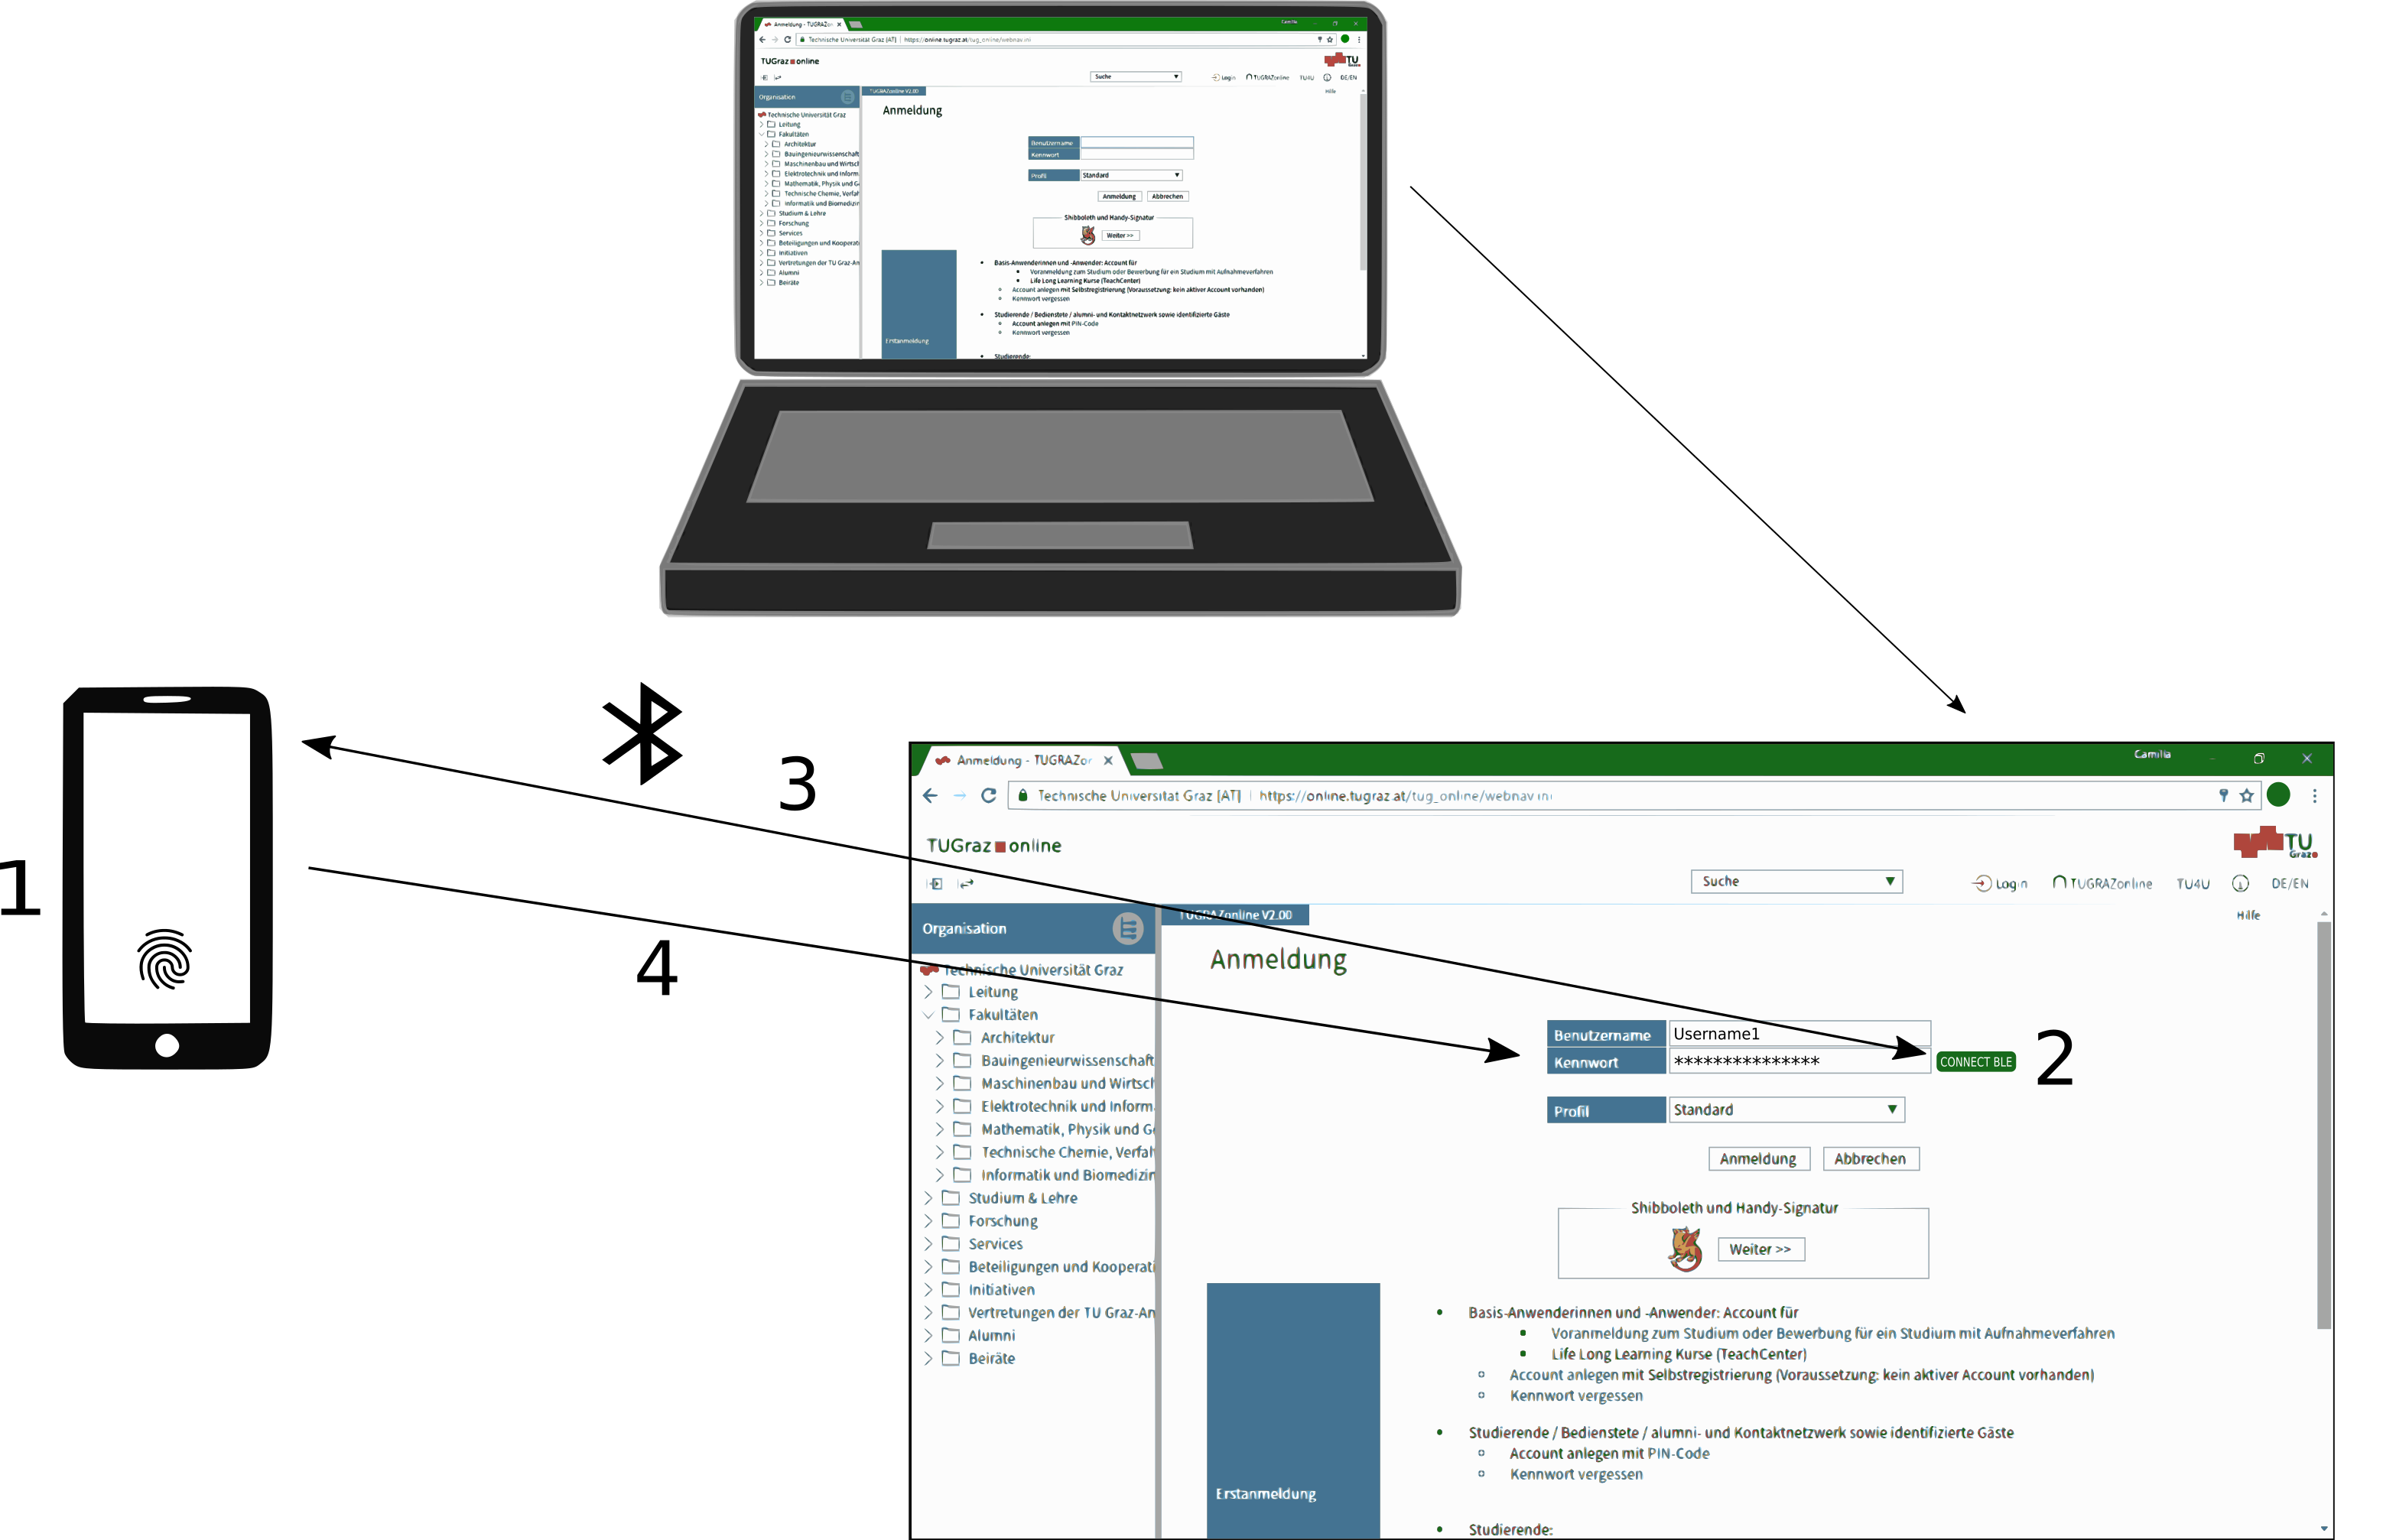
\includegraphics[width=0.9\textwidth]{images/Communication.png}
%
\note{
here see workflow between: \\
First, selects credential and authenticate via fingerprint. successful, advertising.
extension, inject button, step2. button: establish BLE. upon click pairing process step 3. \\
successful pairing, ext allowed read advertised char. step 4 characs contain username and password. ext inserts uname and pw directly into the forms \\}
\end{frame}


\begin{frame}[shrink=8]{Requirements}
\begin{columns}[onlytextwidth]
	\begin{column}{0.49\textwidth}
		Application requirements:
		\begin{itemize}
			\item Storage and management of credentials
			\item Encryption and decryption
			\item Authentication through biometrics
		\end{itemize}
	\end{column}
	\begin{column}{0.47\textwidth}
		Extension requirements:
		\begin{itemize}
			\item Injection of a button
			\item Establishing BLE connection
			\item Read and insert characteristics
		\end{itemize}
	\end{column}
\end{columns} 
%
\note{
Before starting defined requirements \\
requ. of app: \\
Secure storage and management like adding, changing and deleting \\
Encryption and decryption of data \\
Authentication through fingerprint\\
requ. of ext:\\
Injection of a button onto the website \\
Establishment of BLE Connection upon button click \\
Reading the advertised characteristics and inserting them into the proper forms \\}
\end{frame}


\begin{frame}{Storage of Credentials}
\vspace{-10mm}
	\begin{columns}[onlytextwidth]
		\begin{column}{0.7\textwidth}
			\begin{itemize}
				\item ORM greenDAO
				\begin{itemize}
					\item Handles storing, deleting, updating tasks.
				\end{itemize}
				\item Database lies in persistent memory.
				\item Only application can access data.
			\end{itemize}
		\end{column}
		\begin{column}{0.3\textwidth}
			\begin{center}
			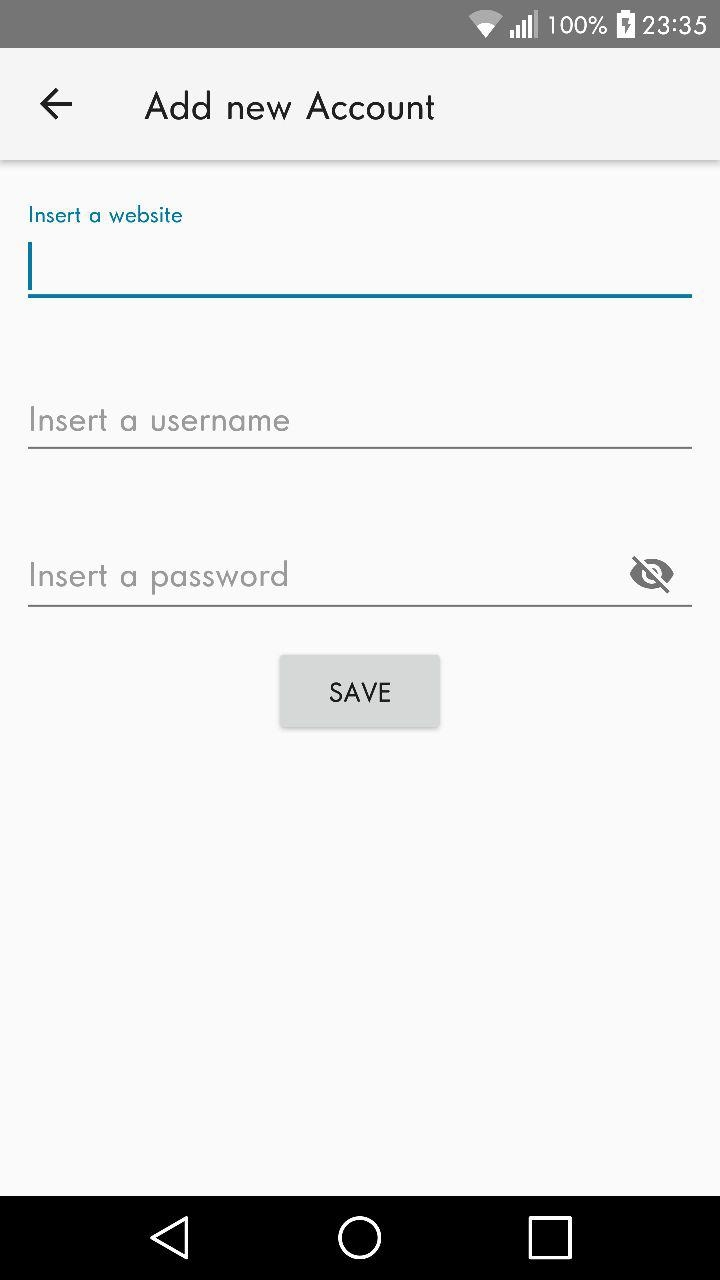
\includegraphics[width=0.8\textwidth]{images/AddAccountActivity.jpg} \\
			\end{center}
		\end{column}
	\end{columns}
%
\note{
To store credentials needed suitable database structure. \\
Decided object-relational mapping framew greenDAO. manages all database related tasks: storing, deleting, updating, querying etc. compared other frameworks, straightforward and intuitive to use. \\
database lies persistent memory and only be accessed from our app. \\}
\end{frame}


\begin{frame}{Encryption of Credentials}
\vspace{-5mm}
\begin{itemize}
	\item Symmetric key encryption algorithm AES-GCM:
	\begin{itemize}
		\item No distribution of public key component.
		\item Fast execution of computations.
		\item Consumes fewer resources.
		\item GCM provides confidentiality, integrity, and authenticity.
	\end{itemize} 
\end{itemize}
%
\note{
For...decided AES algorithm, GCM as cipher mode. \\
because all encryption on phone, no distribution of public part. same key used for both\\
advantages of symmetric key algorithms compared to asymmetric: that it also efficient, secure, provide faster execution of computation, consume fewer such as memory \& processor time. \\
GCM as our cipher mode provides \\}
\end{frame}


\begin{frame}{Storage of Cryptographic Key}
\vspace{-5mm}
	\begin{itemize}
	\item AndroidKeystore stores cryptographic keys.
	\item Only application that created key can access it.
	\item Key is stored in Trusted Execution Environment (TEE).
		\begin{itemize}
		\item TEE depends on device manufacturer.
		\item Data cannot be extracted from the TEE.
		\end{itemize}
\end{itemize}
%
\note{
Store key securely rely on AndroidKeystore system, lets app store/manage keys, no other app access\\
A specific realization of the AndroidKeystore provides a hardware-based security feature: the Trusted Execution Environment. \\
availability TEE depends manufacturer. \\
On devices equipped Qualcomm processor with TrustZone Technology, AKS automatically stored in tee, ensures data not extracted. \\
Represents sec. option to store keys. tee not supported, the key stored system provided emulated software environment. however, both: keys removed when delete app. \\}
\end{frame}


\begin{frame}{Authentication through Biometrics}
\vspace{-10mm}
	\begin{columns}[onlytextwidth]
		\begin{column}{0.7\textwidth}
			\begin{itemize}
			\item Authentication via fingerprint when: 
			\begin{itemize}
				\item Accessing credentials
				\item Sending credentials
			\end{itemize}
			\item Protection of unintentional distribution.
			\end{itemize}
		\end{column}
		\begin{column}{0.3\textwidth}
			\begin{center}
			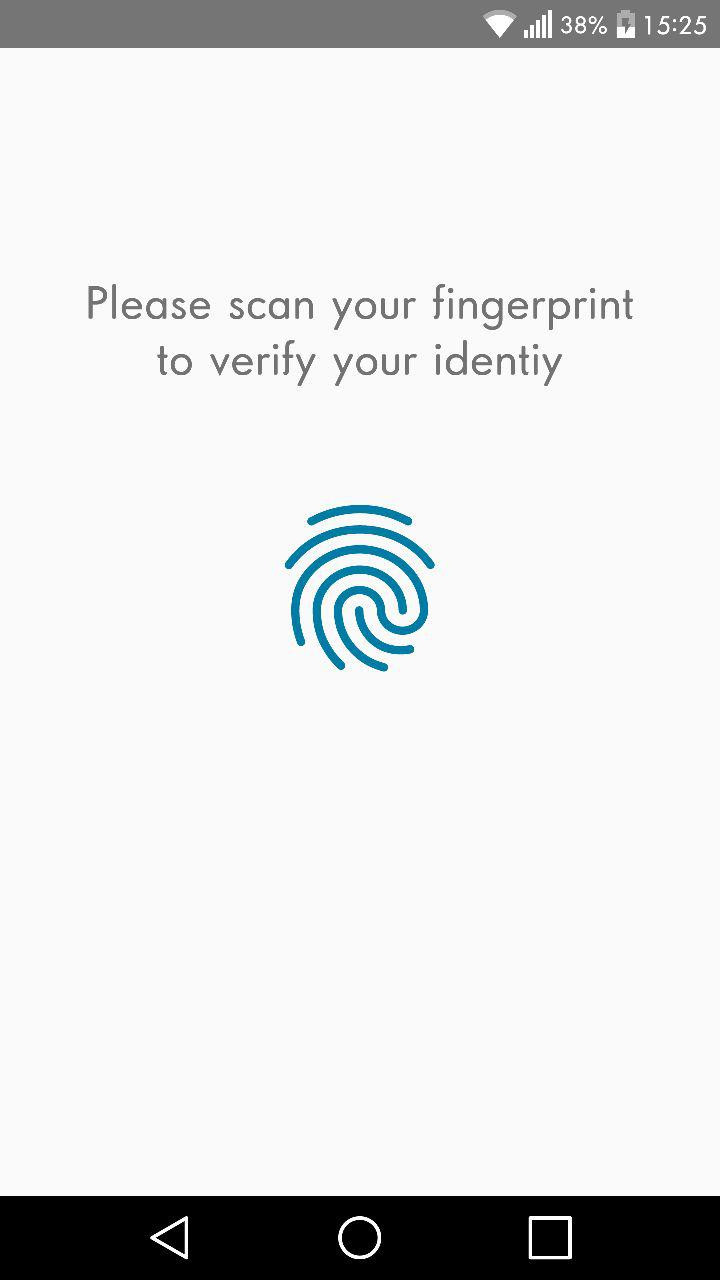
\includegraphics[width=0.8\textwidth]{images/AuthenticationScreenNew.jpg} \\
			\end{center}
		\end{column}
	\end{columns}
%
\note{
to protect credentials, app requires biometric authentication. as biometric auth: use  fingerprint. \\
whenever access/send cred., fingerprint authentication required. upon each new request - needs to re-authenticate. \\
mechanism protects unintentional distribution. Risk threatened sec. reduced the user left their phone unattended with open application.\\}
\end{frame}


\begin{frame}{Chrome Browser Extension}
\begin{itemize}
	\item Establish connection with BLE device.
	\item Extension acts as client and receives data.
	\item Insert data into forms.
	\item Modification of DOM.
\end{itemize}
%
\note{
implemented an extension, chrome introduced dedic. web bt API, support ble conn. website communicate ble devices e.g. heart rate mon. \\
typically ble device advertise and mobile phone consumes., here roles reversed. mobile phone is ble device that advertises. acts as server.\\
extension impl. GATT client retrieve characteristics sent from app. \\ ext. reads values and fills. \\
also modifies the document object model. inject button on website.: initiate connection process between\\
Now guide you through the finished solution of this project: \\}
\end{frame}


\begin{frame}{}
\vfill
\centering
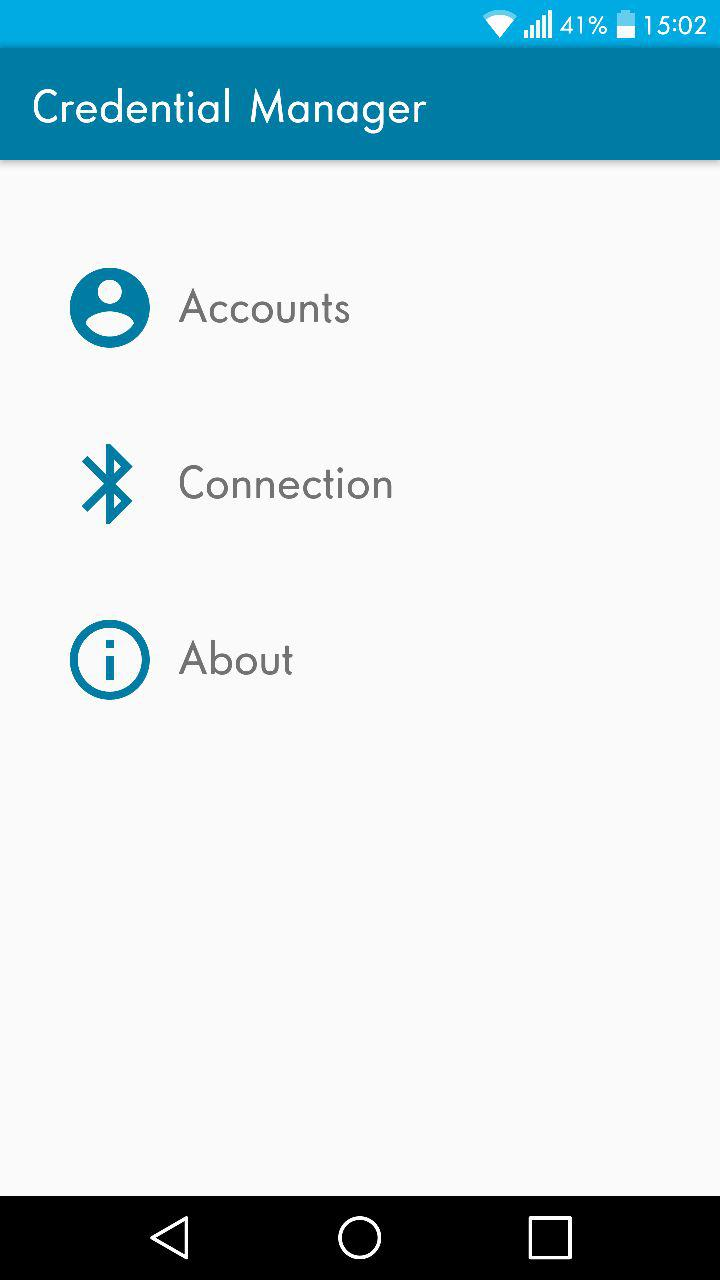
\includegraphics[width=0.31\textwidth]{images/MainActivityNew.jpg}
\hspace{0.1cm}
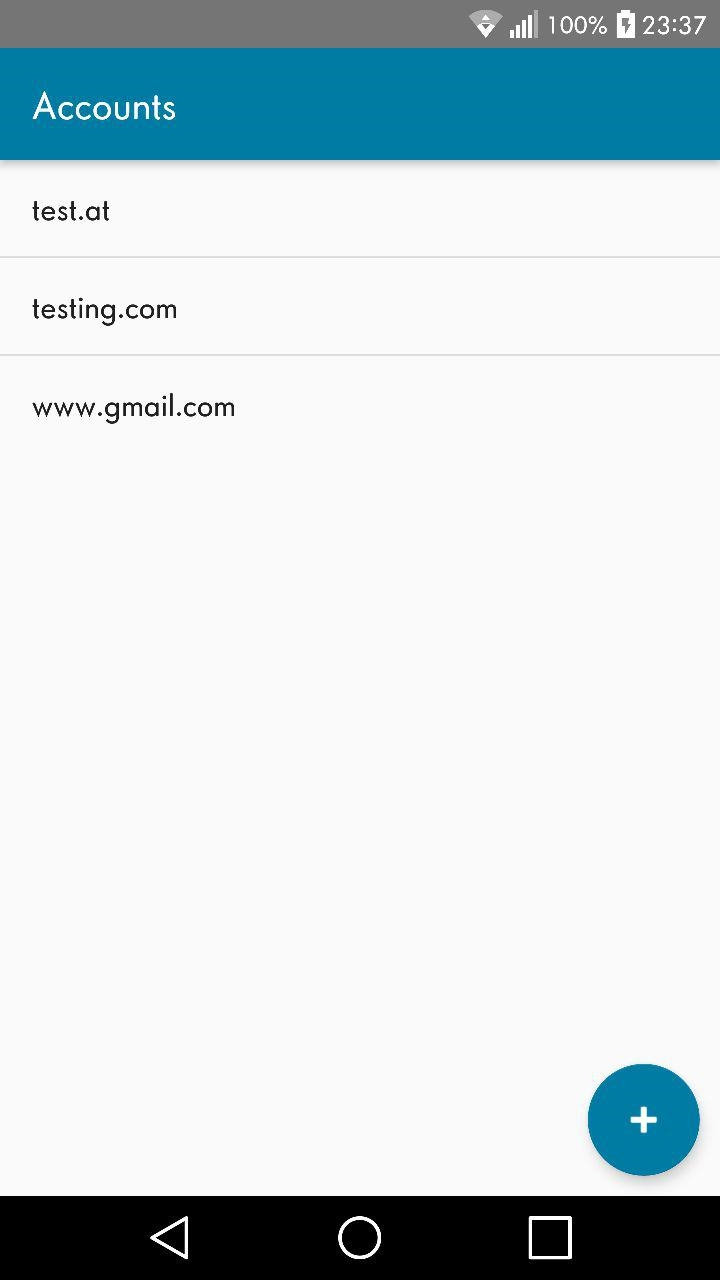
\includegraphics[width=0.31\textwidth]{images/ShowAccountsActivity.jpg}
\hspace{0.1cm}
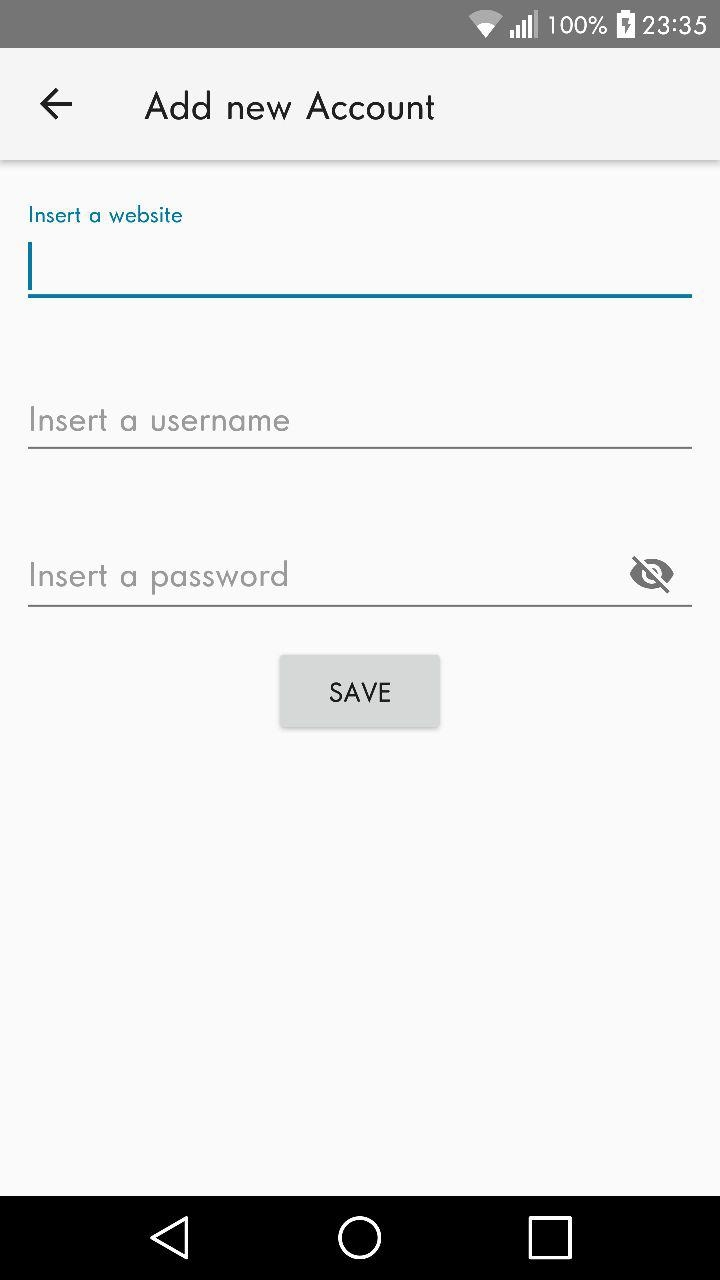
\includegraphics[width=0.31\textwidth]{images/AddAccountActivity.jpg}
\vfill
%
\note{
}
\end{frame}


\begin{frame}{}
\vfill
\centering
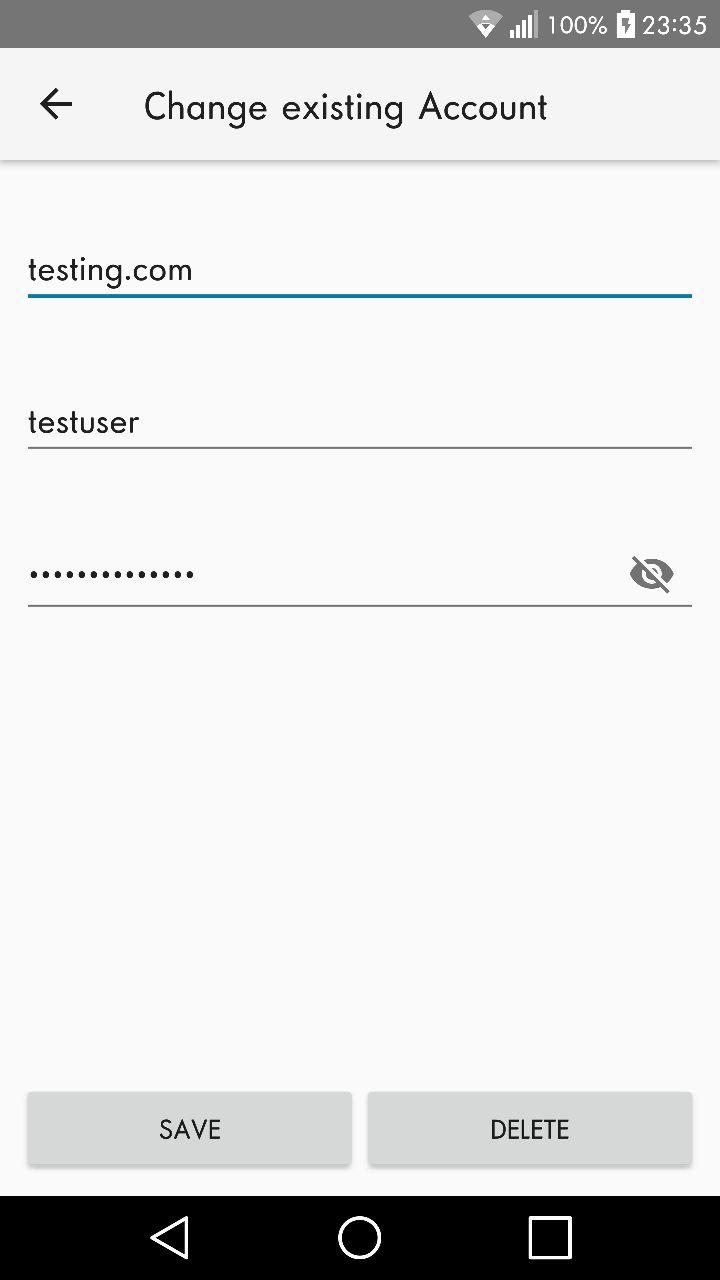
\includegraphics[width=0.31\textwidth]{images/ChangeAccountActivity.jpg}
\hspace{1cm}
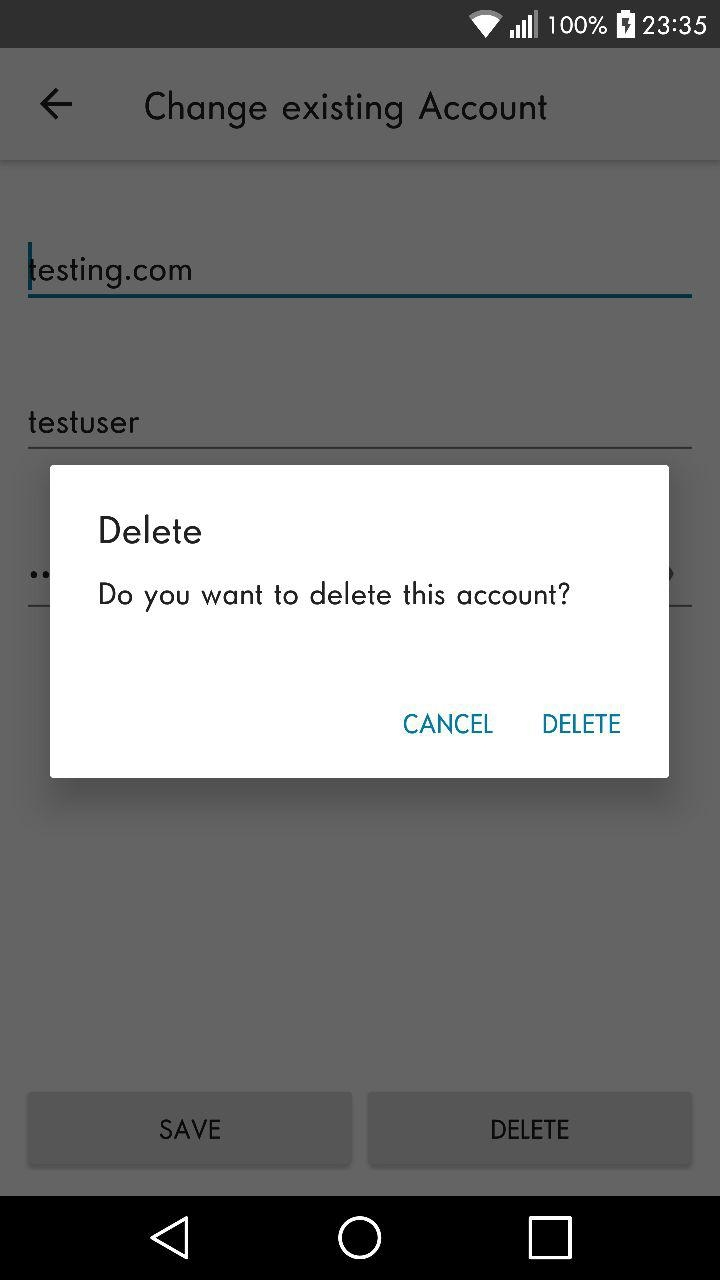
\includegraphics[width=0.31\textwidth]{images/DeleteAccount.jpg}
\vfill
%
\note{
}
\end{frame}

\begin{frame}{}
\vfill
\centering
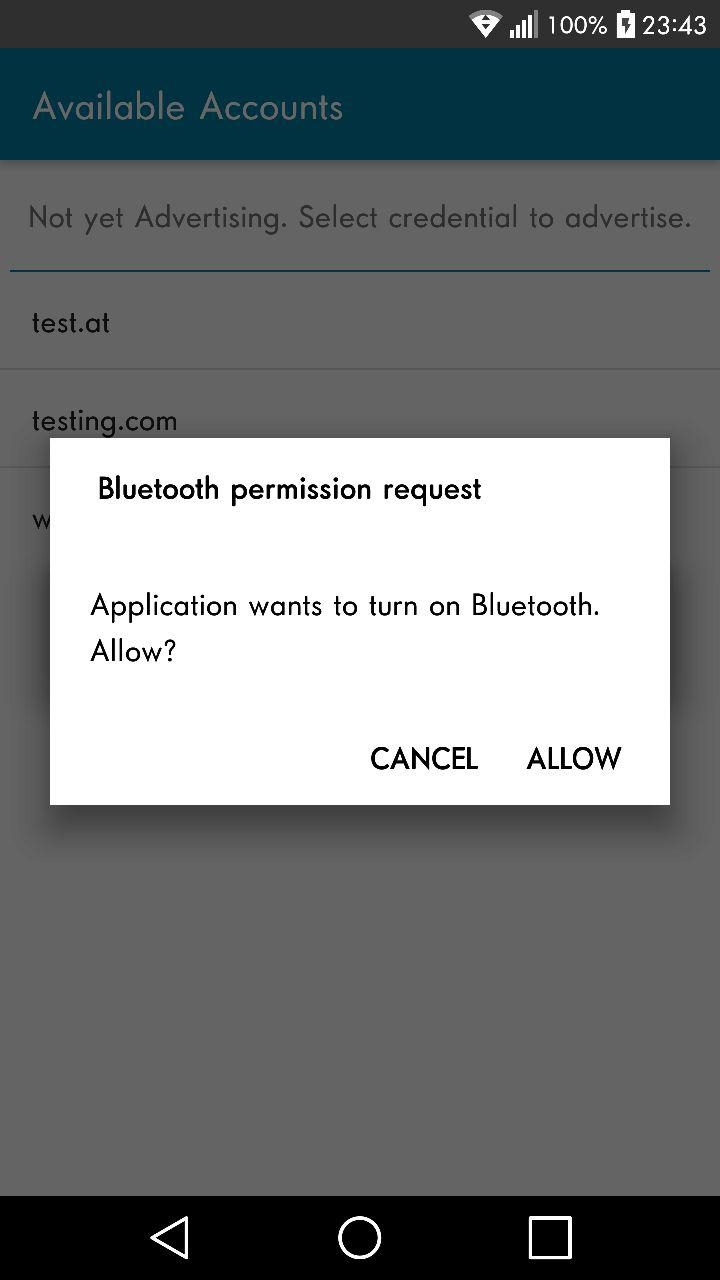
\includegraphics[width=0.31\textwidth]{images/BT_english.jpg}
\hspace{0.1cm}
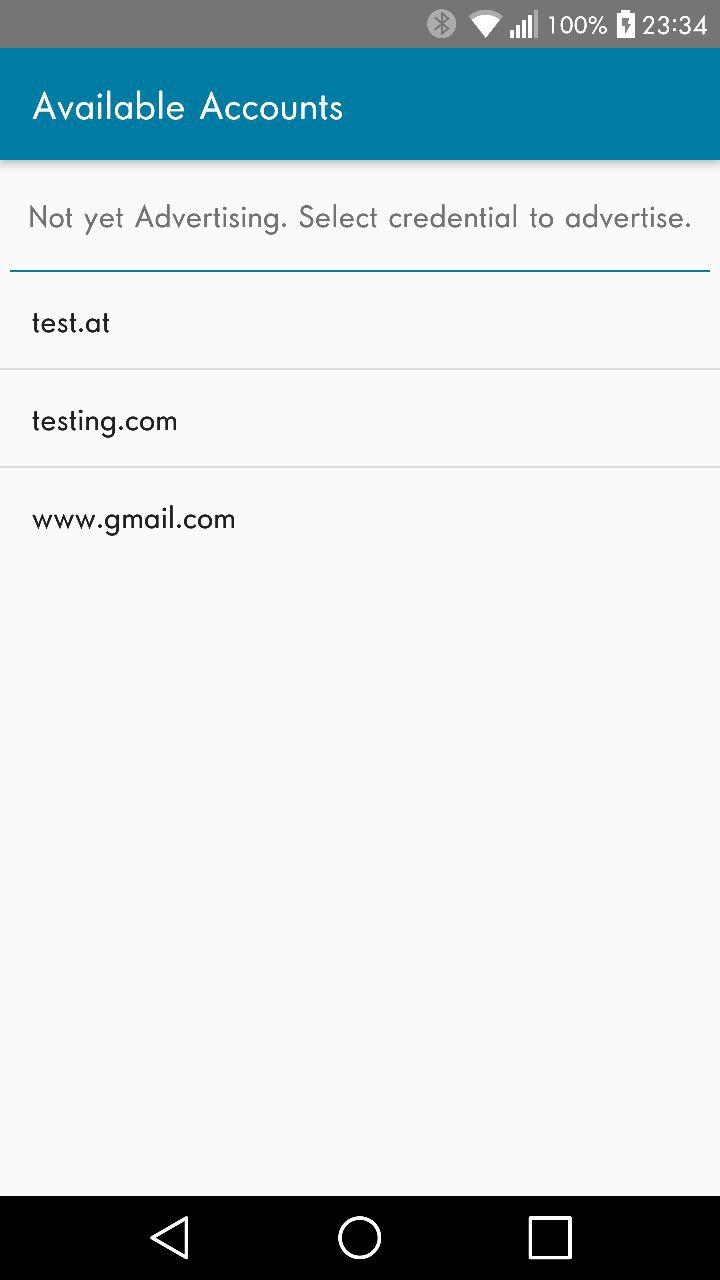
\includegraphics[width=0.31\textwidth]{images/AvailableAccounts.jpg}
\hspace{0.1cm}
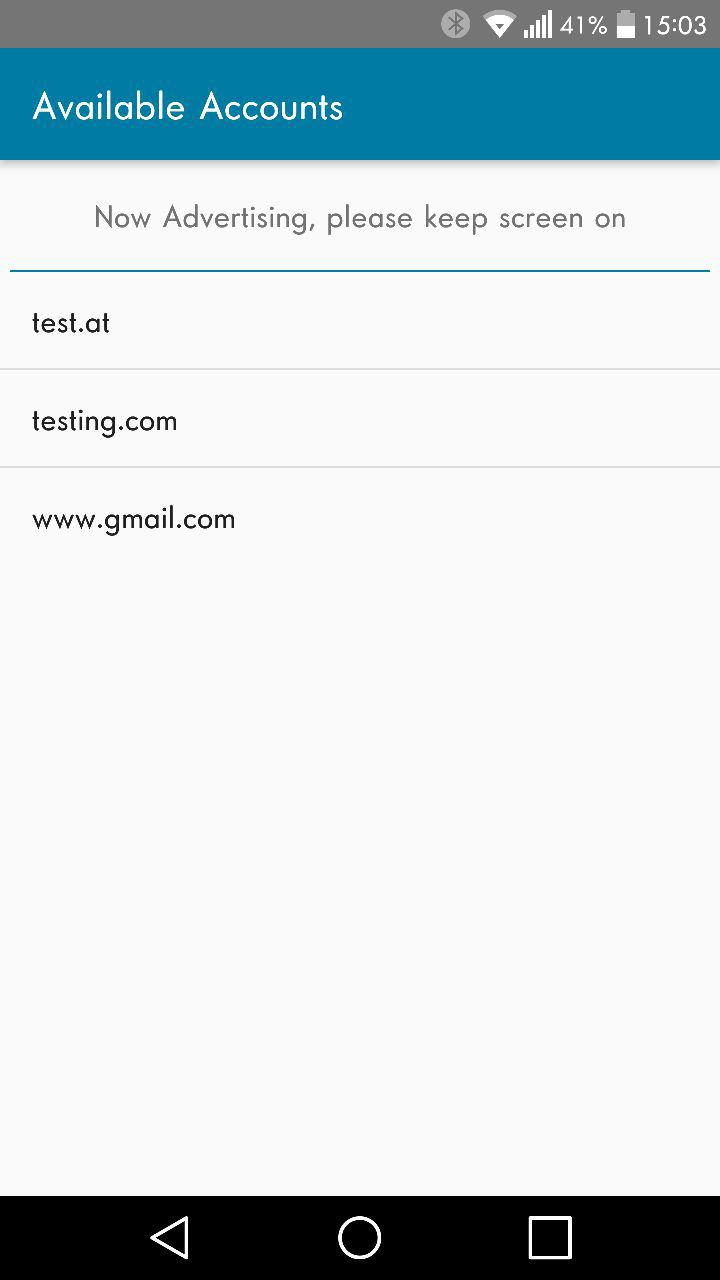
\includegraphics[width=0.31\textwidth]{images/NowAdvertising.jpg}
\vfill
%
\note{
}
\end{frame}

\begin{frame}{}
\vfill
\centering
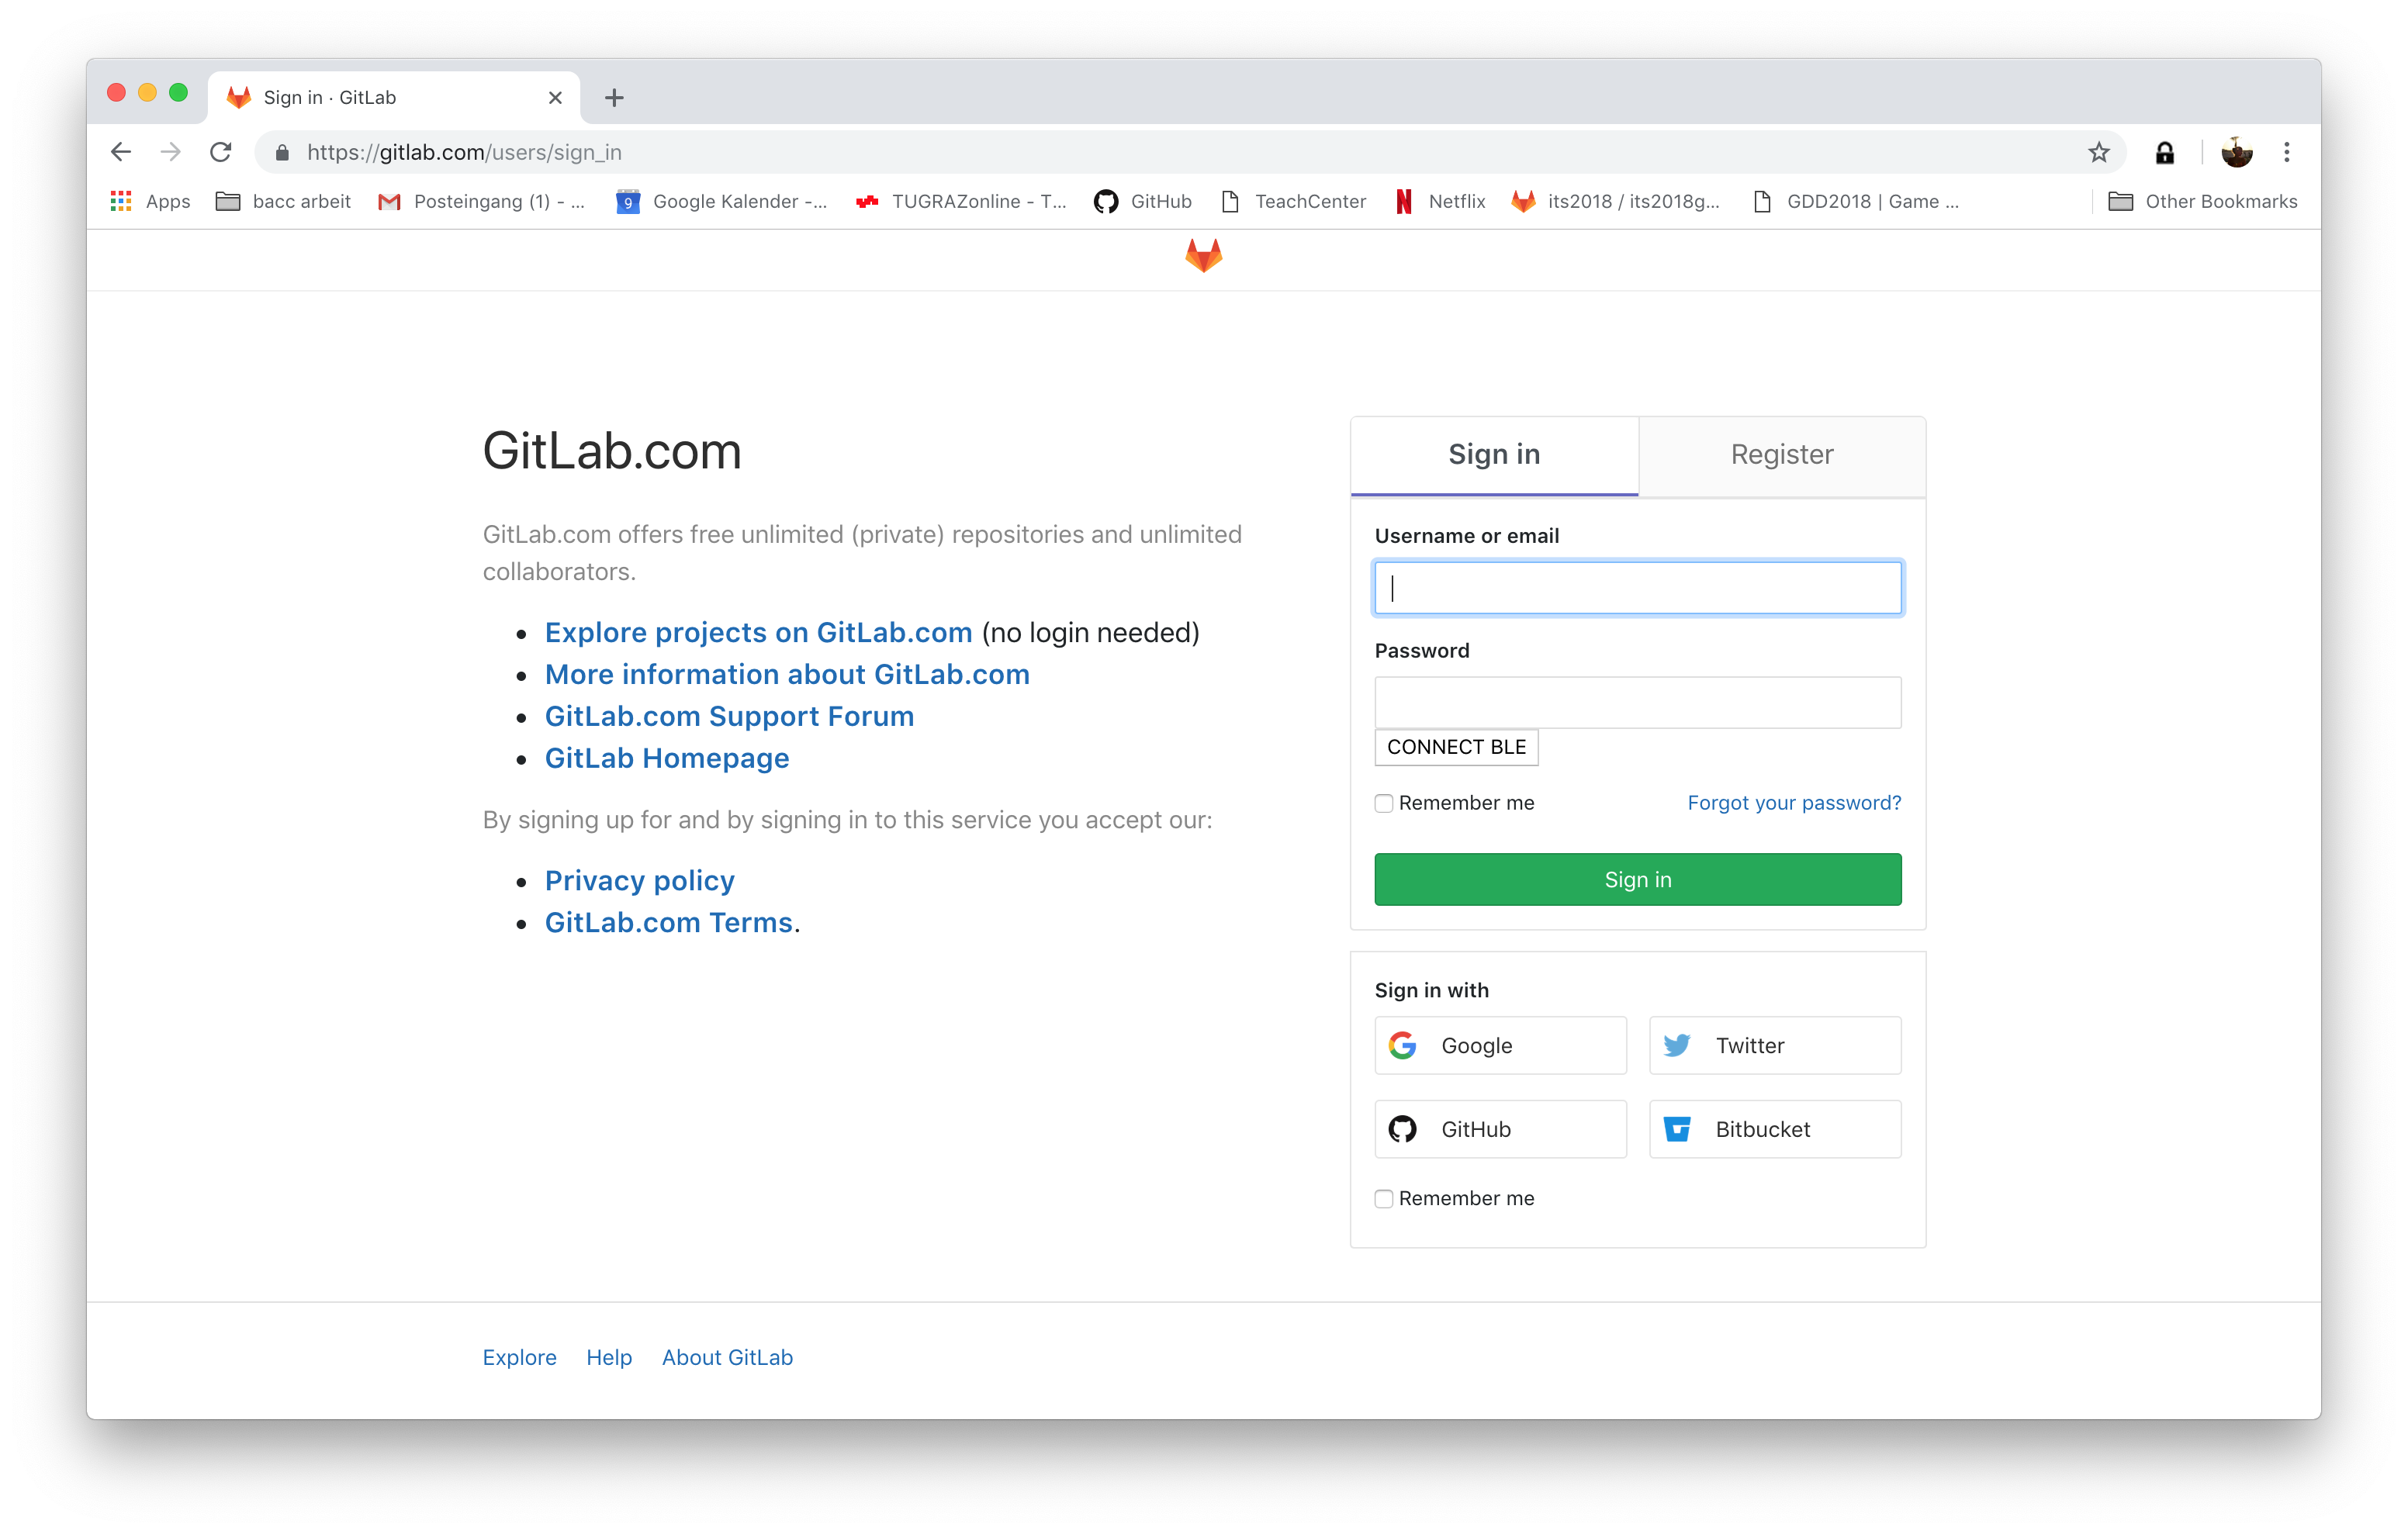
\includegraphics[width=\textwidth]{images/web.png}
\vfill
%
\note{
}
\end{frame}

\section{}
\begin{frame}\frametitle{Summary}
\begin{itemize}
	\item Reduce the risk of unauthorized access by eliminating external dependencies.
	\item Provide availability through a BLE connection.
	\item Securely store credentials on the device.
	\item Authenticate through fingerprint.
\end{itemize}
%
\note{
by eliminate exter. depend. we reduced risk unauthorized access \\
provide availability with ble connection to transfer data to web browser\\
data stored on device and key in the hardware-backed environment provided by the AKS, where extraction is almost infeasible. \\
Distribution accomplished BLE connection between. access and transfer of credentials done fingerp. auth. \\ fingerprint, provide reasonable security maintaining usability. so risk of using insecure PINs and patterns is reduced \\
would like to thank you for \\}
\end{frame}


%%%%%%%%%%%%%%%%%%%%%%%%%%%%%%%%%%%%%%%%%%%%%%%%%%%%%%%%%%%%%%%%%%%%%%%%%%%%

\section*{}
\begin{frame}[shrink=50]{References}
\vspace{-10mm}
\begin{enumerate}
	\item R.Abel, “Android password managers not as secure as desktop counterparts.“ https://www.scmagazine.com/home/security-news/android-password-managers-not-as-secure-as-desktop-counterparts/ \\
	\item C. Cimpanu, “Password managers can be tricked into believing that malicious Android apps are legitimate“ https://www.zdnet.com/article/password-managers-can-be-tricked-into-believing-that-malicious-android-apps-are-legitimate/ \\
	\item W. Wei, “9 Popular Password Manager Apps Found Leaking Your Secrets“ https://thehackernews.com/2017/02/password-manager-apps.html \\
	\item F. Beaufort, “Interact with Bluetooth devices on the Web.” https://developers.google.com/web/updates/2015/07/interact- with-ble-devices-on-the-web \\
	\item U. Ries, “Btlejack: Neues Gratis-Tool zum Belauschen von Bluetooth- Verbindungen.” https://www.heise.de/security/meldung/ Btlejack-Neues-Gratis-Tool-zum-Belauschen-von-Bluetooth- Verbindungen-4134142.html \\
	\item Y. Haider, S. Selvan, “Confidentiality Issues in Cloud Computing and Countermeasures: A Survey“ \\
	\item GreenDAO, “greenDAO: Android ORM for your SQLite database.” http://greenrobot.org/greendao/ \\
	\item Z. Li, W. He, D. Akhawe, and D. Song, “The Emperor’s New Password Manager: Security Analysis of Web-based Password Managers,” in Proceedings of the 23rd USENIX Security Symposium \\
\end{enumerate}
\end{frame}

%%%%%%%%%%%%%%%%%%%%%%%%%%%%%%%%%%%%%%%%%%%%%%%%%%%%%%%%%%%%%%%%%%%%%%%%%%%%

%\section{Motivation}
%%--------------------
%\begin{frame}
%\frametitle{Ziele der ersten Vorlesung}
%Einführung in die KORE
%\begin{itemize}
%	\item Geschichte der KORE kennen lernen
%	\item Aufgaben der KORE und Einordnung in das betriebliche Rechnungswesen verstehen
%	\item Wertebenen im Rechnungswesen unterscheiden
%\end{itemize}
%
%Grundlagen der KORE
%\begin{itemize}
%	\item Kostenwürfel als Hilfsmittel verwenden
%	\item Überleitung von externem zu internem Rechnungswesen durchführen
%\end{itemize}
%\end{frame}

%%%%%%%%%%%%%%%%%%%%%%%%%%%%%%%%%%%%%%%%%%%%%%%%%%%%%%%%%%%%%%%%%%%%%%%%%%%%

%\section{Related Work}
%%--------------------
%\begin{frame}
%\frametitle{Titel der Folie\\maximal zwei Zeilen}
%Text Ebene 1
%\begin{itemize}
%	\item Zweite Ebene
%	\begin{itemize}
%		\item Dritte Ebene
%		\begin{itemize}
%			\item Vierte Ebene
%		\end{itemize}
%	\end{itemize}
%\end{itemize}
%\end{frame}

%%%%%%%%%%%%%%%%%%%%%%%%%%%%%%%%%%%%%%%%%%%%%%%%%%%%%%%%%%%%%%%%%%%%%%%%%%%%

%\section{Finished Project}
%%--------------------
%\begin{frame}[fragile]
%	\frametitle{Android Application}
%	\begin{spacing}{1}
%	\begin{semiverbatim}
%SUCHE (A,x)
%1: i = 0
%2: WHILE i<n
%3:     i = i+1
%4:     \alert{IF A[i]=x THEN RETURN i}
%5: ELSE RETURN -1
%	\end{semiverbatim}
%	\end{spacing}
%\end{frame}

%%%%%%%%%%%%%%%%%%%%%%%%%%%%%%%%%%%%%%%%%%%%%%%%%%%%%%%%%%%%%%%%%%%%%%%%%%%%

%\section{Spalten und Grafiken}
%%--------------------
%\begin{frame}
%	\frametitle{Zwei Inhalte Links/Rechts\\Wahlweise Text/Grafik}
%	\begin{columns}[onlytextwidth]
%		\begin{column}{0.5\textwidth}
%			\begin{itemize}
%				\item Lorem ipsum dolor sit amet, consectetur 
%				\item adipisicing elit, sed do eiusmod tempor 
%				\item incididunt ut labore et dolore magna aliqua. 
%				\item Ut enim ad minim veniam, quis nostrud 
%			\end{itemize}
%		\end{column}
%		\begin{column}{0.5\textwidth}
%			\begin{center}
%			
\includegraphics[width=0.5\textwidth]{logo.pdf}\\
%			Grafik in Spalte 2
%			\end{center}
%		\end{column}
%	\end{columns}
%\end{frame}
%
%\section{Weitere Beispielfolien}
%
%\begin{frame}
%\frametitle{Titel der Folie\\maximal zwei Zeilen}
%	Ein Link:
%	\begin{center}
%		\url{http://www.tugraz.at}		
%	\end{center}
%\end{frame}
%
%\sectionheader[Untertitel]{Abschnittsbeginn}

%%%%%%%%%%%%%%%%%%%%%%%%%%%%%%%%%%%%%%%%%%%%%%%%%%%%%%%%%%%%%%%%%%%%%%%%%%%%

%\section{Zusammenfassung}
%%--------------------
%\begin{frame}
%	\frametitle{Zusammenfassung}
%	\begin{itemize}
%		\item Punkt 1
%		\item Punkt 2
%		\item Punkt 3
%	\end{itemize}
%\end{frame}

%%%%%%%%%%%%%%%%%%%%%%%%%%%%%%%%%%%%%%%%%%%%%%%%%%%%%%%%%%%%%%%%%%%%%%%%%%%%
\end{document}
%%%%%%%%%%%%%%%%%%%%%%%%%%%%%%%%%%%%%%%%%%%%%%%%%%%%%%%%%%%%%%%%%%%%%%%%%%%%

%% EOF
